\documentclass[submit]{harvardml}

% Put in your full name and email address.
\name{Melissa Yu}
\email{melissayu@college.harvard.edu}

% List any people you worked with.
\collaborators{%
  Alex Lin
}


% You don't need to change these.
\course{CS281-F17}
\assignment{Assignment \#0, v 1.0}
\duedate{5:00pm Sept. 8th}
\newcommand{\attr}[1]{\textsf{#1}}
\usepackage[OT1]{fontenc}
\usepackage[colorlinks,citecolor=blue,urlcolor=blue]{hyperref}
\usepackage[pdftex]{graphicx}
\usepackage{fullpage}
\usepackage{palatino}
\usepackage{amsfonts}
\usepackage{amsmath}
\usepackage{amssymb}
\usepackage{color}
\usepackage{todonotes}
\usepackage{listings}
\usepackage{common}
\usepackage{bm}
\usepackage{enumitem}
\usepackage{tikz}
\usepackage{xifthen}
\usepackage{soul}
\usepackage{url}
\usepackage[mmddyyyy,hhmmss]{datetime}
\definecolor{verbgray}{gray}{0.9}
% Some useful macros.
\newcommand{\R}{\mathbb{R}}
\newcommand{\E}{\mathbb{E}}
\newcommand{\cov}{\text{cov}}
\renewcommand{\v}[1]{\mathbf{#1}}

\begin{document}
\begin{center}
    {\Large Homework 0: Preliminary}
\end{center}

\subsection*{Introduction}

There is a mathematical component and a programming component to this homework.
Please submit your PDF and Python files to Canvas, and push all of your work
to your GitHub repository. If a question requires you to make any plots,
please include those in the writeup.

This assignment is intended to ensure that you have the background required for CS281,
and have studied the mathematical review notes provided in section.
You should be able to answer the problems below \textit{without} complicated calculations.
All questions are worth $70/6 = 11.\bar{6}$ points unless stated otherwise.

\newpage



%%%%%%%%%%%%%%%%%%%%%%%%%%%%%%%%%%%%%%%%%%%%%%%%%%%%%%%%
%%%%%%%%%%%%%%%%%% PROBLEM 1 %%%%%%%%%%%%%%%%%%%%%%%%%%%
%%%%%%%%%%%%%%%%%%%%%%%%%%%%%%%%%%%%%%%%%%%%%%%%%%%%%%%%
\section*{Variance and Covariance}
\begin{problem}
Let $X$ and~$Y$ be two independent random variables.

\begin{enumerate}[label=(\alph*)]
\item Show that the independence of~$X$ and~$Y$ implies that their
covariance is zero.

\item Zero covariance \textit{does not} imply independence between two
      random variables. Give an example of this.

\item For a scalar constant~$a$, show the following two properties:
\begin{align*}
  \E(X + aY) &= \E(X) + a\E(Y)\\
  \var(X + aY) &= \var(X) + a^2\var(Y)
\end{align*}
\end{enumerate}
\end{problem}

\begin{enumerate}
	\item[(a)] As shown in math review, we have $\E(XY) = \E(X)\E(Y)$ for independent variables $X$ and $Y$. Expanding the expression for covariance, we obtain the desired result:
	\begin{align*}
	\cov (X, Y) &= \E\left[(X - \E(X)) (Y - \E(Y))\right] \\
	&= \E\left[(XY - \E(X)Y - \E(Y)X + \E(X)\E(Y)\right] \\
	&= \E(XY) - \E(X)\E(Y) & \text{by linearity of expectation} \\
	&= 0
	\end{align*}
	
	\item[(b)] Take $X\sim\mathcal{N}(0, 1)$ and $Y\sim X^2$. Then, we have the covariance
	\begin{align*}
	\cov(X, Y) &= \E\left[(X - \E(X)) (X^2 - \E(X^2))\right] \\
	&= \E(X^3) \\
	&= 0,
	\end{align*}
	where $\E(X^3)$ can be shown to be 0 by evaluating the third derivative of the moment generating function for the standard normal at 0.
	
	\item[(c)] For the case where $X$ and $Y$ are discrete R.V.s, we have:
	\begin{align*}
	\E(X + aY) &= \sum_{x, y} (x + ay) P(X = x, Y = y) \\
	&= \sum_{x, y} x P(X = x, Y = y) + \sum_{x, y} ay P(X = x, Y = y) \\
	&= \sum_{x} x P(X = x) + \sum_{y} ay P(Y = y) \\
	&= \E(X) + a\E(Y)
	\end{align*}
	The proof for continuous R.V.s uses integrals instead of summations, and is analogous.
	\begin{align*}
	\var(X + aY) &= \E\left[(X + aY)^2\right] - \E\left[X + aY\right]^2 \\
	&= \E\left[X^2 + 2aXY + a^2Y^2\right] - \left(\E(X)^2 + 2a\E(X)\E(Y) + a^2\E(Y)^2\right) \\
	&= \E(X^2) - \E(X)^2 + a^2(\E(Y^2) - \E(Y)^2) \\
	&= \var(X) + a^2\var(Y)
	\end{align*}
	
\end{enumerate}


\newpage
%%%%%%%%%%%%%%%%%%%%%%%%%%%%%%%%%%%%%%%%%%%%%%%%%%%%%%%%
%%%%%%%%%%%%%%%%%% PROBLEM 2 %%%%%%%%%%%%%%%%%%%%%%%%%%%
%%%%%%%%%%%%%%%%%%%%%%%%%%%%%%%%%%%%%%%%%%%%%%%%%%%%%%%%
\section*{Densities}
\begin{problem}
Answer the following questions:
\begin{enumerate}[label=(\alph*)]
  \item Can a probability density function (pdf) ever take values greater than 1?
  \item Let $X$ be a univariate normally distributed random variable with mean 0
        and variance $1/100$. What is the pdf of $X$?
  \item What is the value of this pdf at 0?
  \item What is the probability that $X = 0$?
  \item Explain the discrepancy.
\end{enumerate}
\end{problem}

\begin{enumerate}
	\item[(a)] Yes; the pdf is just a measure of the \textit{relative} probability of a value.
	
	\item[(c)] Substituting into the pdf for the normal, we have:
	\[
	X\sim \mathcal{N}(0, 1/100) 
	\implies f_X(x) 
	= \frac{10}{\sqrt{2\pi}}\exp\left(-50x^2\right)
	\]
	
	\item[(c)] $f_X(0) = \frac{10}{\sqrt{2\pi}}$
	
	\item[(d)] $P(X = 0) = 0$
	
	\item[(e)] The real probability of a continuous R.V. equaling an exact value is 0 (there are infinitely many values on the support), but the relative probability of this event is not 0.
\end{enumerate}



\newpage
%%%%%%%%%%%%%%%%%%%%%%%%%%%%%%%%%%%%%%%%%%%%%%%%%%%%%%%%
%%%%%%%%%%%%%%%%%%%% PROBLEM 3 %%%%%%%%%%%%%%%%%%%%%%%%%
%%%%%%%%%%%%%%%%%%%%%%%%%%%%%%%%%%%%%%%%%%%%%%%%%%%%%%%%
\section*{Conditioning and Bayes' rule}
\begin{problem}
  Let $\v \mu \in \R^m$ and
  $\v \Sigma, \v \Sigma' \in \R^{m \times m}$.  Let $X$ be an
  $m$-dimensional random vector with
  $X \sim \mathcal{N}(\v \mu, \v \Sigma)$, and let $Y$ be a
  $m$-dimensional random vector such that
  $Y \given X \sim \mathcal{N}(X, \v \Sigma')$. Derive the
  distribution and parameters for each of the following.

\begin{enumerate}[label=(\alph*)]
  \item The unconditional distribution of $Y$.

  \item The joint distribution for the pair $(X,Y)$.

\end{enumerate}

Hints:
\begin{itemize}
\item You may use without proof (but they are good advanced exercises)
  the closure properties of multivariate normal distributions. Why is
  it helpful to know when a distribution is normal?
\item Review Eve's and Adam's Laws, linearity properties of
  expectation and variance, and Law of Total Covariance.

\end{itemize}

\end{problem}

\begin{enumerate}
	\item[(a)] From the closure properties for a multinomial distribution, we have that $Y$ is distributed MVN with some mean and covariance matrix. To completely specify the distribution, we need only compute these two parameters:
	\begin{align*}
	\E(Y) &= \E(\E(Y\given X))  = \E(X) = \mu \\
	\cov(Y, Y) &= \E(\var(Y\given X)) + \var(\E(Y\given X)) \\
	&= \E(\v\Sigma') + \var(X) \\
	&= \v\Sigma' + \v{\Sigma}
	\end{align*}
	Thus,
	\[Y\sim\mathcal{N}(\mu, \v{\Sigma + \v{\Sigma'}})\]
	
	\item[(b)] We can understand this joint distribution as the vector 
	$Z = \begin{bmatrix} X \\ Y\end{bmatrix}$. As before, we know this is distributed MVN by the closure properties. Then, the expected value is simply
	\[ \E(Z) 
	= \begin{bmatrix} \E(X) \\ \E(Y)\end{bmatrix} 
	= \begin{bmatrix} \mu \\ \mu\end{bmatrix} \]
	Similarly, the covariance matrix of $Z$ can be expressed as:
	\[ \cov(Z, Z)
	= \begin{bmatrix} \cov(X, X) & \cov(X, Y) \\ \cov(Y, X) & \cov(Y, Y)\end{bmatrix} \]
	We can use the law of total covariance to compute the off-diagonal covariances:
	\begin{align*}
	\cov(X, Y) &= \E(\cov(X, Y\given X)) + \cov(\E(X\given X), \E(Y\given X)) \\
	&= 0 + \cov(X, X),
	\end{align*}
	where the covariance of $X$ and $Y$ given $X$ is 0, since the two are independent given $X$. Thus, we have the joint distribution
	\[
	\begin{bmatrix} X \\ Y\end{bmatrix} \sim
	\mathcal{N}\left(
	\begin{bmatrix} \mu \\ \mu\end{bmatrix},
	\begin{bmatrix} \v\Sigma & \v\Sigma \\ \v\Sigma & \v\Sigma + \v\Sigma' \end{bmatrix}
	\right)
	\]
\end{enumerate}

\newpage
%%%%%%%%%%%%%%%%%%%%%%%%%%%%%%%%%%%%%%%%%%%%%%%%%%%%%%%%
%%%%%%%%%%%%%%%%% PROBLEM 4 %%%%%%%%%%%%%%%%%%%%%%%%%%%%
%%%%%%%%%%%%%%%%%%%%%%%%%%%%%%%%%%%%%%%%%%%%%%%%%%%%%%%%
\section*{I can Ei-gen}
\begin{problem}
    Let $\v X \in \R^{n \times m}$.
    \begin{enumerate}[label=(\alph*)]
        \item What is the relationship between the $n$ eigenvalues
              of $\v X \v X^T$ and the $m$ eigenvalues of $\v X^T \v X$?
        \item Suppose $\v X$ is square (i.e., $n=m$) and symmetric.
              What does this tell you about the eigenvalues of $\v X$?
              What are the eigenvalues of $\v X + \v I$, where $\v I$ is the identity matrix?
        \item Suppose $\v X$ is square, symmetric, and invertible.
			  What are the eigenvalues of $\v X^{-1}$?
	\end{enumerate}
	Hints:
	\begin{itemize}
		\item Make use of singular value decomposition and the properties
			  of orthogonal matrices. Show your work.
		\item Review and make use of (but do not derive) the spectral theorem.
	\end{itemize}
\end{problem}

\begin{enumerate}
	\item[(a)] Let the SVD of $\v X$ be $\v U\v\Sigma \v V^T$, where $\v U$ and $\v V$ are orthogonal and $\v \Sigma$ is diagonal. Making use of the fact that $\v V \v V^T = \v I$ for any orthogonal matrix $\v V$, we have the following diagonalizations:
	\begin{align*}
	\v X\v X^T &= \v U\v\Sigma\v V^T\v V\v\Sigma^T\v U^T = \v U\v\Sigma\v\Sigma^T\v U^T \\
	\v X^T\v X &= \v V\v\Sigma^T \v U^T\v U\v\Sigma\v V^T = \v V\v\Sigma^T\v\Sigma\v V^T
	\end{align*}
	Since $\v\Sigma$ is a diagonal matrix, $\v\Sigma^T\v\Sigma$ and $\v\Sigma\v\Sigma^T$ have the same values on their diagonals, except for zero padding. Thus, we conclude that the two matrices have the same non-zero eigenvalues, with the larger matrix having additional zero-eigenvalues.
	
	\item[(b)] By the spectral theorem, the eigenvalues of $\v X$ are all real and correspond to $n$ orthogonal eigenvectors. For any eigenvalue $\lambda$ with eigenvector $v$ of $\v X$, we have $\v X v = \lambda v \implies (\v X + \v I) v = (\lambda + 1) v$. Thus, the eigenvalues of the new matrix are found by adding one to the eigenvalues of the original matrix.
	
	\item[(c)] For any eigenvalue $\lambda$ with eigenvector $v$ of $\v X$, we have 
	\[\v X v = \lambda v \implies \v X^{-1} \v X v = \v X^{-1} \lambda v \implies \v X^{-1} v = \frac{1}{\lambda} v\]
	Thus, the eigenvalues of $\v X^{-1}$ are simply the reciprocals of the original eigenvalues.
\end{enumerate}


\newpage
%%%%%%%%%%%%%%%%%%%%%%%%%%%%%%%%%%%%%%%%%%%%%%%%%%%%%%%%%%
%%%%%%%%%%%%%%%%%%% PROBLEM 5 %%%%%%%%%%%%%%%%%%%%%%%%%%%%
%%%%%%%%%%%%%%%%%%%%%%%%%%%%%%%%%%%%%%%%%%%%%%%%%%%%%%%%%%
\section*{Vector Calculus}
\begin{problem}
  Let $\v x, \v y \in \R^m$ and $\v A \in \R^{m \times m}$. Please derive from
  elementary scalar calculus the following useful properties. Write
  your final answers in vector notation.
\begin{enumerate}[label=(\alph*)]
    \item What is the gradient with respect to $\v x$ of $\v x^T \v y$?
    \item What is the gradient with respect to $\v x$ of $\v x^T \v x$?
    \item What is the gradient with respect to $\v x$ of $\v x^T \v A \v x$?
\end{enumerate}
\end{problem}

\begin{enumerate}
	\item[(a)] First, we observe that
	\[\frac{\partial \v x^T\v y}{\partial x_k} = \frac{\partial \sum_{i=1}^{m} x_i y_i}{\partial x_k} = y_k\]
	Combining, we obtain
	\begin{align*}
	\frac{\partial \v x^T\v y}{\partial \v x} &= \begin{bmatrix}
	\frac{\partial \v x^T\v y}{\partial x_1} \\
	\vdots \\
	\frac{\partial \v x^T\v y}{\partial x_m}
	\end{bmatrix} 
	= \begin{bmatrix}
	y_1 \\
	\vdots \\
	y_m
	\end{bmatrix} = \v y
	\end{align*}
	
	\item[(b)] Again, we expand the dot product as
	\[\frac{\partial \v x^T\v x}{\partial x_k} = \frac{\partial \sum_{i=1}^{m} x_i^2}{\partial x_k} = 2x_k\]
	Thus,
	\begin{align*}
	\frac{\partial \v x^T\v x}{\partial \v x} &= \begin{bmatrix}
	\frac{\partial \v x^T\v x}{\partial x_1} \\
	\vdots \\
	\frac{\partial \v x^T\v x}{\partial x_m}
	\end{bmatrix} = \begin{bmatrix}
	2x_1 \\
	\vdots \\
	2x_m
	\end{bmatrix} = 2 \v x
	\end{align*}
	
	\item[(c)] Noting that $\v x^T\v A\v x = \langle \v A\v x, \v x\rangle = \sum_{i=1}^{m} \sum_{j=1}^m x_i A_{ij} x_j$, we have:
	\[
	\frac{\partial \v x^T\v A\v x}{\partial x_k} = \sum_{j=1}^m (A_{jk} + A_{kj}) x_j
	\]
	As before, we obtain:
	\begin{align*}
	\frac{\partial \v x^T\v A\v x}{\partial \v x} &= \begin{bmatrix}
	\frac{\partial \v x^T\v A\v x}{\partial x_1} \\
	\vdots \\
	\frac{\partial \v x^T\v A\v x}{\partial x_m}
	\end{bmatrix} 
	= \begin{bmatrix}
	\sum_{j=1}^m (A_{j1} + A_{1j}) x_j \\
	\vdots \\
	\sum_{j=1}^m (A_{jm} + A_{mj}) x_j \\
	\end{bmatrix} = (\v A + \v A^T) \v x
	\end{align*}
\end{enumerate}

\newpage
%%%%%%%%%%%%%%%%%%%%%%%%%%%%%%%%%%%%%%%%%%%%%%%%%%%%%%%%%%%%
%%%%%%%%%%%%%%%%%%%%% PROBLEM 7 %%%%%%%%%%%%%%%%%%%%%%%%%%%%
%%%%%%%%%%%%%%%%%%%%%%%%%%%%%%%%%%%%%%%%%%%%%%%%%%%%%%%%%%%%
\section*{Gradient Check}
\begin{problem}
  Often after finishing an analytic derivation of a gradient, you will
  need to implement it in code.  However, there may be mistakes -
  either in the derivation or in the implementation. This is
  particularly the case for gradients of multivariate functions.

  \air

  \noindent One way to check your work is to numerically estimate the gradient
  and check it on a variety of inputs. For this problem we consider
  the simplest case of a univariate function and its derivative.  For
  example, consider a function $f(x): \mathbb{R} \to \mathbb{R}$:
$$\frac{d f}{d x} = \underset{\epsilon \to 0} \lim \frac{f(x + \epsilon) - f(x - \epsilon)}{2 \epsilon}$$
\noindent A common check is to evaluate the right-hand side for a small value of
$\epsilon$, and check that the result is similar to your analytic
result.\\

\smallskip

\noindent In this problem, you will implement the analytic and numerical derivatives of the function \[f(x) = \cos(x) + x^2 + e^x.\]

\begin{enumerate}
  \item Implement \texttt{f} in Python (feel free to use whatever \texttt{numpy} or \texttt{scipy} functions you need):
  \begin{lstlisting}[language=python]
  def f(x):
  	return np.cos(x) + x ** 2 + np.exp(x)

  \end{lstlisting}
  \item Analytically derive the derivative of that function, and implement it in Python:
  \begin{lstlisting}[language=python]
  def grad_f(x):
  	return - np.sin(x) + 2 * x + np.exp(x)

  \end{lstlisting}
  \item Now, implement a gradient check (the numerical approximation to the derivative), and by plotting, 
        show that the numerical approximation approaches the analytic as \texttt{epsilon} 
        $\to 0$ for a few values of $x$:
  \begin{lstlisting}[language=python]
  def grad_check(x, epsilon):
  	return (f(x + epsilon) - f(x - epsilon)) / (2 * epsilon)
	
  \end{lstlisting}
\end{enumerate}
\end{problem}

\newpage
The function implementations are completed above, and can also be found in the python files submitted to Canvas. The graph below shows the difference between the analytic and numerical solutions for various epsilon. As expected, the difference becomes smaller as epsilon goes to 0.

\begin{center}
	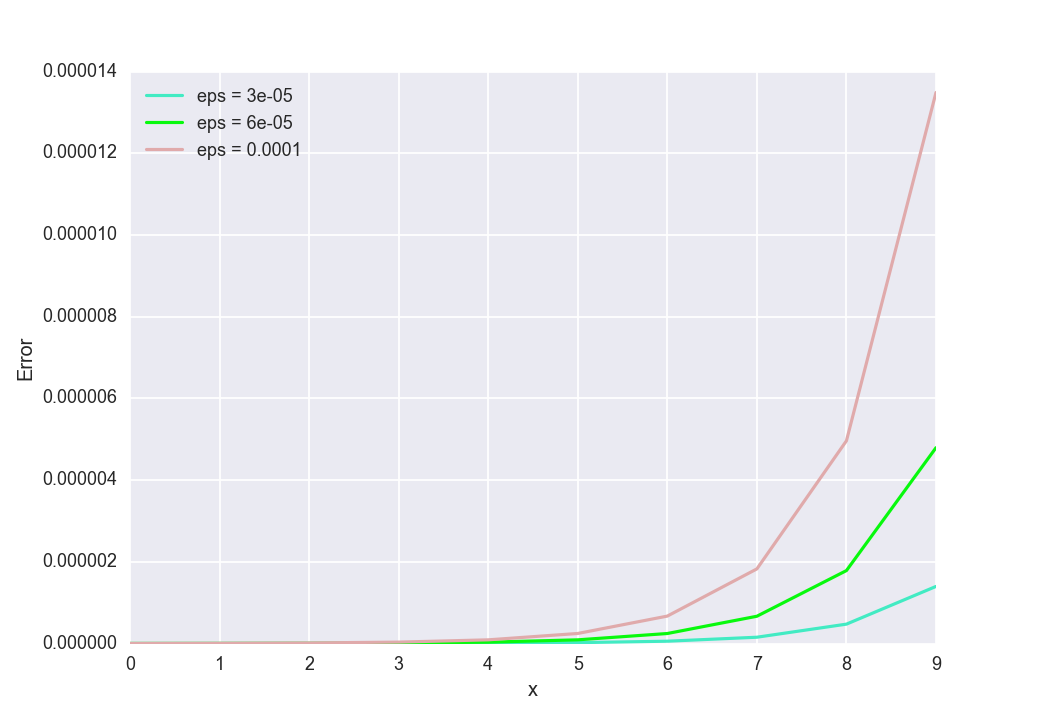
\includegraphics[scale=0.5]{6}
\end{center}

\end{document}
